%-------------------------------------------------------------------------------
% This file provides a skeleton ATLAS document.
%-------------------------------------------------------------------------------
% \pdfoutput=1
% The \pdfoutput command is needed by arXiv/JHEP/JINST to ensure use of pdflatex.
% It should be included in the first 5 lines of the file.
%-------------------------------------------------------------------------------
% Specify where ATLAS LaTeX style files can be found.
\newcommand*{\ATLASLATEXPATH}{latex/}
% Use this variant if the files are in a central location, e.g. $HOME/texmf.
% \newcommand*{\ATLASLATEXPATH}{}
%-------------------------------------------------------------------------------
\documentclass[UKenglish,texlive=2016]{\ATLASLATEXPATH atlasdoc}
% The language of the document must be set: usually UKenglish or USenglish.
% british and american also work!
% Commonly used options:
%  texlive=YYYY          Specify TeX Live version (2016 is default).
%  atlasstyle=true|false Use ATLAS style for document (default).
%  coverpage             Create ATLAS draft cover page for collaboration circulation.
%                        See atlas-draft-cover.tex for a list of variables that should be defined.
%  cernpreprint          Create front page for a CERN preprint.
%                        See atlas-preprint-cover.tex for a list of variables that should be defined.
%  PAPER                 The document is an ATLAS paper (draft).
%  CONF                  The document is a CONF note (draft).
%  PUB                   The document is a PUB note (draft).
%  BOOK                  The document is of book form, like an LOI or TDR (draft)
%  txfonts=true|false    Use txfonts rather than the default newtx - needed for arXiv submission.
%  paper=a4|letter       Set paper size to A4 (default) or letter.

%-------------------------------------------------------------------------------
% Extra packages:
\usepackage{\ATLASLATEXPATH atlaspackage}

\makeatletter
\def\blx@maxline{77}
\makeatother

% Commonly used options:
%  biblatex=true|false   Use biblatex (default) or bibtex for the bibliography.
%  backend=biber         Use the biber backend rather than bibtex.
%  subfigure|subfig|subcaption  to use one of these packages for figures in figures.
%  minimal               Minimal set of packages.
%  default               Standard set of packages.
%  full                  Full set of packages.
%-------------------------------------------------------------------------------
% Style file with biblatex options for ATLAS documents.
\usepackage{\ATLASLATEXPATH atlasbiblatex}

% Package for creating list of authors and contributors to the analysis.
\usepackage{\ATLASLATEXPATH atlascontribute}

% Useful macros
\usepackage{\ATLASLATEXPATH atlasphysics}
% See doc/atlas_physics.pdf for a list of the defined symbols.
% Default options are:
%   true:  journal, misc, particle, unit, xref
%   false: BSM, heppparticle, hepprocess, hion, jetetmiss, math, process, other, texmf
% See the package for details on the options.

% Files with references for use with biblatex.
% Note that biber gives an error if it finds empty bib files.
\addbibresource{ToyMCJetTutorial.bib}
\addbibresource{bibtex/bib/ATLAS.bib}

% Paths for figures - do not forget the / at the end of the directory name.
\graphicspath{{logos/}{figures/}}

% Add you own definitions here (file ToyMCJetTutorial-defs.sty).
\usepackage{ToyMCJetTutorial-defs}

%-------------------------------------------------------------------------------
% Generic document information
%-------------------------------------------------------------------------------

% Title, abstract and document 
%-------------------------------------------------------------------------------
% This file contains the title, author and abstract.
% It also contains all relevant document numbers used by the different cover pages.
%-------------------------------------------------------------------------------

% Title
\AtlasTitle{Monte Carlo and Jet Tutorial}

% Author - this does not work with revtex (add it after \begin{document})
%\author{Samuel Meehan}

% Authors and list of contributors to the analysis
% \AtlasAuthorContributor also adds the name to the author list
% Include package latex/atlascontribute to use this
% Use authblk package if there are multiple authors, which is included by latex/atlascontribute
% \usepackage{authblk}
% Use the following 3 lines to have all institutes on one line
% \makeatletter
% \renewcommand\AB@affilsepx{, \protect\Affilfont}
% \makeatother
% \renewcommand\Authands{, } % avoid ``. and'' for last author
% \renewcommand\Affilfont{\itshape\small} % affiliation formatting
% \AtlasAuthorContributor{First AtlasAuthorContributor}{a}{Author's contribution.}
% \AtlasAuthorContributor{Second AtlasAuthorContributor}{b}{Author's contribution.}
% \AtlasAuthorContributor{Third AtlasAuthorContributor}{a}{Author's contribution.}
% \AtlasContributor{Fourth AtlasContributor}{Contribution to the analysis.}
\author[a]{Samuel Meehan}
\author[b]{Fiona Pons}
\affil[a]{University of Washington}
\affil[b]{Heidelberg KIP}


% If a special author list should be indicated via a link use the following code:
% Include the two lines below if you do not use atlasstyle:
% \usepackage[marginal,hang]{footmisc}
% \setlength{\footnotemargin}{0.5em}
% Use the following lines in all cases:
% \usepackage{authblk}
% \author{The ATLAS Collaboration%
% \thanks{The full author list can be found at:\newline
%   \url{https://atlas.web.cern.ch/Atlas/PUBNOTES/ATL-PHYS-PUB-2016-007/authorlist.pdf}}
% }

% Draft version:
% Should be 1.0 for the first circulation, and 2.0 for the second circulation.
% If given, adds draft version on front page, a 'DRAFT' box on top of each other page, 
% and line numbers.
% Comment or remove in final version.
%\AtlasVersion{0.1}

% ATLAS reference code, to help ATLAS members to locate the paper
%\AtlasRefCode{GROUP-2016-XX}

% ATLAS note number. Can be an COM, INT, PUB or CONF note
% \AtlasNote{ATLAS-CONF-2016-XXX}
% \AtlasNote{ATL-PHYS-PUB-2016-XXX}
% \AtlasNote{ATL-COM-PHYS-2016-XXX}

% CERN preprint number
% \PreprintIdNumber{CERN-PH-2016-XX}

% ATLAS date - arXiv submission; usually filled in by the Physics Office
% \AtlasDate{\today}

% ATLAS heading - heading at top of title page. Set for TDR etc.
% \AtlasHeading{ATLAS ABC TDR}

% arXiv identifier
% \arXivId{14XX.YYYY}

% HepData record
% \HepDataRecord{ZZZZZZZZ}

% Submission journal and final reference
% \AtlasJournal{Phys.\ Lett.\ B.}
% \AtlasJournalRef{\PLB 789 (2014) 123}
% \AtlasDOI{}

% Abstract - % directly after { is important for correct indentation
\AtlasAbstract{%
  This tutorial is meant to introduce students to the concept of Monte Carlo in the context
  of studying hadronic jets at the LHC.  It is written with the intent of being a self-guided
  introduction to research and data analysis in high energy physics.
}

%-------------------------------------------------------------------------------
% The following information is needed for the cover page. The commands are only defined
% if you use the coverpage option in atlasdoc or use the atlascover package
%-------------------------------------------------------------------------------

% List of supporting notes  (leave as null \AtlasCoverSupportingNote{} if you want to skip this option)
% \AtlasCoverSupportingNote{Short title note 1}{https://cds.cern.ch/record/XXXXXXX}
% \AtlasCoverSupportingNote{Short title note 2}{https://cds.cern.ch/record/YYYYYYY}
%
% OR (the 2nd option is deprecated, especially for CONF and PUB notes)
%
% Supporting material TWiki page  (leave as null \AtlasCoverTwikiURL{} if you want to skip this option)
% \AtlasCoverTwikiURL{https://twiki.cern.ch/twiki/bin/view/Atlas/WebHome}

% Comment deadline
% \AtlasCoverCommentsDeadline{DD Month 2016}

% Analysis team members - contact editors should no longer be specified
% as there is a generic email list name for the editors
% \AtlasCoverAnalysisTeam{Peter Analyser, Susan Editor1, Jenny Editor2, Alphonse Physicien}

% Editorial Board Members - indicate the Chair by a (chair) after his/her name
% Give either all members at once (then they appear on one line), or separately
% \AtlasCoverEdBoardMember{EdBoard~Chair~(chair), EB~Member~1, EB~Member~2, EB~Member~3}
% \AtlasCoverEdBoardMember{EdBoard~Chair~(chair)}
% \AtlasCoverEdBoardMember{EB~Member~1}
% \AtlasCoverEdBoardMember{EB~Member~2}
% \AtlasCoverEdBoardMember{EB~Member~3}

% A PUB note has readers and not an EdBoard -- give their names here (one line or several entries)
% \AtlasCoverReaderMember{Reader~1, Reader~2}
% \AtlasCoverReaderMember{Reader~1}
% \AtlasCoverEdBoardMember{Reader~2}

% Editors egroup
% \AtlasCoverEgroupEditors{atlas-GROUP-2016-XX-editors@cern.ch}

% EdBoard egroup
% \AtlasCoverEgroupEdBoard{atlas-GROUP-2016-XX-editorial-board@cern.ch}


% Author and title for the PDF file
\hypersetup{pdftitle={ATLAS document},pdfauthor={The ATLAS Collaboration}}

%-------------------------------------------------------------------------------
% Content
%-------------------------------------------------------------------------------
\begin{document}

\maketitle

%\tableofcontents


\section{Introduction}
One of the most commonly used tools to construct models in high energy physics (HEP) is Monte Carlo (MC) simulation.  
This form of model building is applicable from the description of fundamental processes to the behavior of large detector systems and electronics.  The reason for using Monte Carlo simularion is rooted both in the inherent random nature of the systems under study as well as the ability to describe a complex system by the composition of many smaller processes.  

There is extensive literature concerning the design of various types of Monte Carlo models, and extending what you learn here to those applications is your responsibility.  In this tutorial, an introduction to MC modelling is explored in the context of describing the physics of \textit{jets}~\cite{Ellis:1276292,Ellis:2007ib} and the Large Hadron Collider (LHC)~\cite{Evans:2008zzb} and how we study them using detectors called calorimeters~\cite{Proudfoot:2006tr}.



\section{What is a Jet?}
\label{sec:whatisjet}
The LHC is a particle accelerator designed to collide protons at extremely high energies, where the kinetic energy of the proton is $\sim10^{}12$ times as great as its rest mass energy.  At such high energies, when two protons collide, the interaction that occurs takes place between the parton constituents of the proton (i.e. quarks ($q$) and gluons ($g$)).  When such a collision occurs, a large number of processes may result.  The exact process that occurs depends on the configuration of the initial state of the collision from proton-1 and proton-2 ($qq$, $qg$, $gg$) and the energy of each of these partons\footnote{Though these may seem fixed by the choice we make to collide protons at a fixed energy, there is still an inherent degree of randomness that is taken into account when conducting real simulations which is explored in one of the extensions of this project in Section~\ref{sec:extensions}.}.  However, there are other aspects of the collision process that proceed differently on a collision-by-collision basis even if the initial state of the collision is the same.  In some cases, the incoming partons may produce a $Z$ boson or a photon.  In other cases, it may produce a Higgs boson which decays to two photons.  It is precisely this random nature of what is produced that is the aim of the type of quantum physics being studied at the LHC and is described by what is called quantum field theory.  

In quantum field theory, the exact process which occurs is unpredictable but will almost assuredly be accompanied by the associated production of additional quarks and gluons.  Unfortunately, describing the behavior of quarks and gluons is a sub-field of quantum field theory, called quantum chromo-dynamics (QCD), that is very challenging, primarily because the strength of the interaction is very large~\cite{wilcek:nobel}.  For those performing theoretical calculations, this strong interaction means that the standard techniques used to describe the dynamics of systems that involve quarks and gluons cannot yet be described with the same level of precision that we can describe the interaction of electrons and photons, their electromagnetic counterparts.  For experimentalists working at the LHC, the strong interaction means that the production of a single quark or gluon, which often occurs in conjunction with something more interesting like the production of a Higgs boson, does not lead to the detection of a single particle in the detector.  Instead, the first quark or gluon that is produced will itself spawn the production of more quarks and gluons which themselves will spawn more quarks and gluons eventually leading to the creation of a spray of partons.  This is called the \textit{parton shower} and is represented by the final state portion of the diagram in Figure~\ref{fig:shower} until the gray ovals.  This process will continue until the energy of the first parton has been subdivided so far that the large set of partons that is has spawned are low enough energy that it is energetically favorable not to spawn more partons but rather to bind together into stable composite particles, hadrons.  This is called \textit{hadronization} and is represented by the gray ovals in Figure~\ref{fig:shower} which creates stable particles, the yellow circles on the final state.  These hadrons are what fly into the apparatus constructed around the collision point and are detected in what are called calorimeters\footnote{Even the behavior of the detector is somewhat random and modelled by MC simulation.  How to model this is one of the topics to be explored in one of the extensions of this project in Section~\ref{sec:extensions}.} and are observed s a collimated spray of particles called a ``jet''.

It is precisely these two processes, the parton shower and hadronization, that make the study of quarks and gluons challenging at the LHC because the production of a single parton will actually appear in the detector as many particles, collimated in the same generatl direction, all arriving at once.  The detection of a collimated flow of particles of this nature is what is called a \textit{jet}~\cite{Ellis:1276292,Ellis:2007ib}.  Moreover, because calculating the behavior of quarks and gluons in QCD is challenging, there is not even an exact prediction of what such a ``jet'' of particles \textit{should} look like.  Luckily, it is possible to understand the behavior of the parton shower in extreme limits of QCD on which to base a model for how additional partons are created.  Likewise, it is also possible to use similar guiding principles to build a model of how these will eventual bind together into stable hadrons.  In both cases, the model that is used will be simpler than the exact and parameterized in terms of an set of parameters that we choose.  Finally, and most importantly for the purposes of this tutorial, the models used for these two processes both have degrees of randomness resulting from the fact that they describe a quantum process which allows them to be described by a Monte Carlo model.  

\begin{figure}[!ht]
\centering
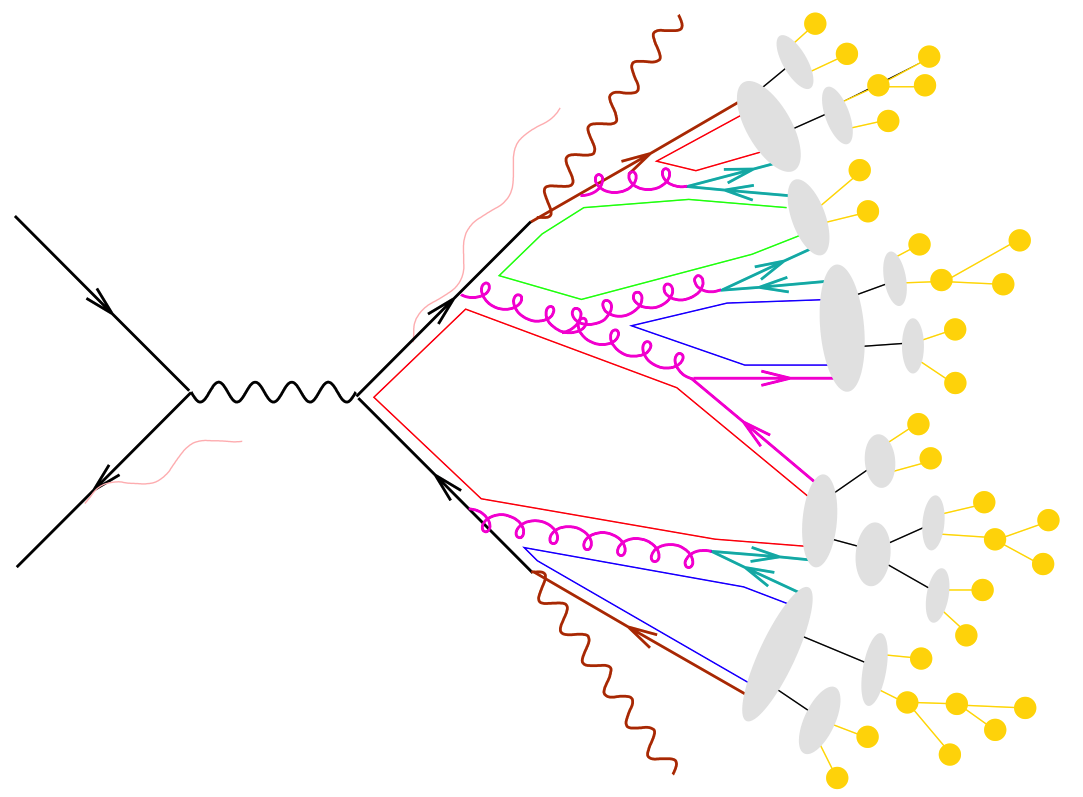
\includegraphics[width=0.6\columnwidth]{figures/ps.png}
\caption{Illustration of the decay of a $W$ or $Z$ boson to a $q\bar{q}$ pair with the subsequent dynamics of the parton shower (red and purple lines) and hadronization (gray clusters
and yellow circles) of the hard partons.  
\label{fig:shower}}
\end{figure}

\subsection{The Parton Shower}
\label{sec:ps}
Describing the evolution of a single partons to many partons by this process of spawning additional partons by strong interactions is impossible to fully describe with the equations of QCD.  However, it can be shown that given an $n$ leg Feynman diagram ($\mathcal{M}_{n}$), the $n+1$ leg Feynman diagram ($\mathcal{M}_{n+1}$) formed by including an additional contribution from a parton \textit{splitting} ($a\rightarrow bc$), as shown in Figure~\ref{fig:diagrams}, scales as:

\begin{equation}
|\mathcal{M}_{n+1}|^2 \sim \frac{1}{\theta^{2}} C_{A} F(z) |\mathcal{M}_{n}|^2
\end{equation}

\begin{figure}[!ht]
 \centering
 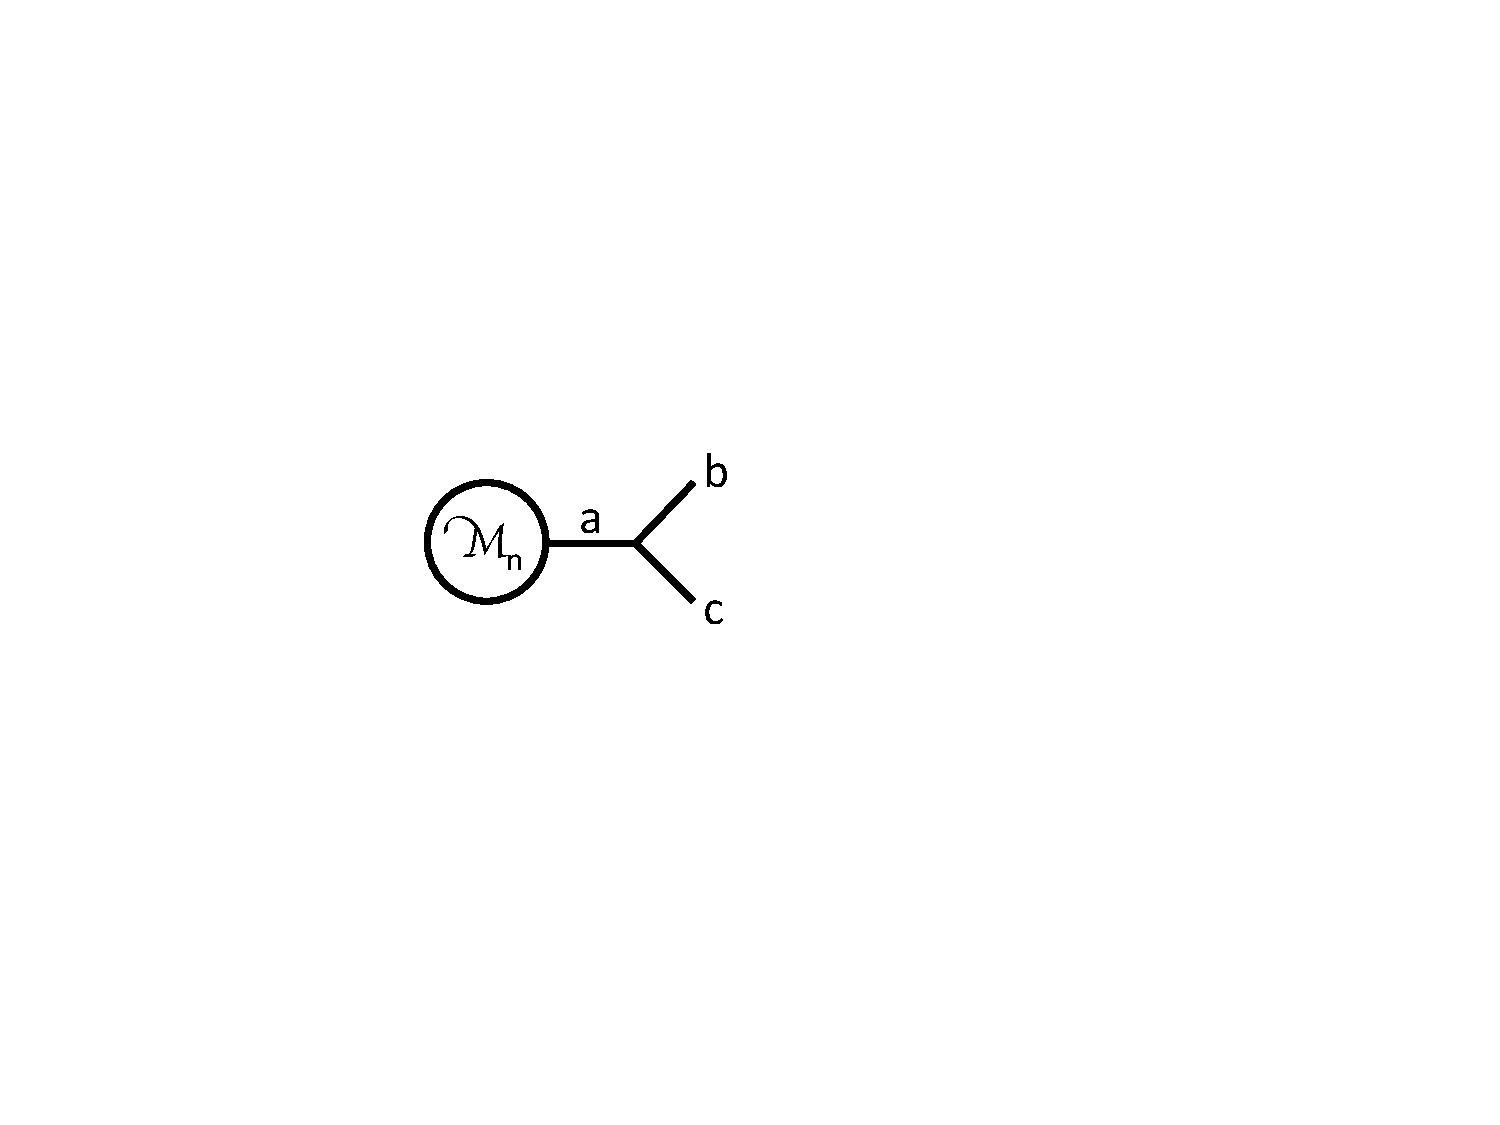
\includegraphics[width=0.3\columnwidth]{figures/diagram}
 \caption{The Feynman diagram representing an $n+1$ leg matrix element process $\mathcal{M}_{n+1}$, build from an $n$ leg process $\mathcal{M}_{n}$ and an additional parton splitting.
 \label{fig:diagrams}}
\end{figure}

\noindent
where $z=\frac{E_{b}}{E_{a}}$ is the relative energy of the more energetic parton after the splitting to that of the initial parton and $\theta$ is the opening angle of the splitting between parton $b$ and parton $c$.  In this model of a single emission, the parameters $z$ and $\theta$ are real physical


There are three key features that emerge from this equation that dictate the first order evolution of jets.  The first concerns the function $F(z)$, related to the $abc$ splitting vertex and depends whether the vertex is a $ggg$, $qqg$, or $gqq$ vertex.  For the $gqq$ vertex, this function is well defined for all values of $z$ but for the $ggg$ and $qqg$ vertices a singularity exists for an emission of $z=0$ or $z=1$, meaning that radiation coming from these splittings are preferentially low energy, ``soft'', and generally follow a functional form of $1/z$.  Second, the $1/\theta$ singularity common to all vertices implies that splitting are preferentially at small angles, ``collinear''.  The third key feature is that in addition to the soft and collinear nature of the splittings, the splittings do not depend on the azimuthal angle around the axis of propagation of parton $a$.  These three features lead to the intuition that the resulting partonic energy pattern coming from the initial parton that was produced will generally be azimuthally symmetric around the its initial direction with an energetic central core and some amount of less energetic radiation distributed further out.

\subsection{Hadronization}
\label{sec:had}
The physics of the parton shower is modelled by a limiting case of the full model of QCD.  However, when the energy scale of the parton shower becomes low enough, the same model of QCD, involving quarks and gluons interacting at vertices is no longer valid.  Instead, it is necessary for the physical description to use composite particles, hadrons, to describe the physics.  Therefore, it is necessary to make a transition from an ensemble of partons to an ensemble of hadrons.  Understanding this transition is not well understood from first principles and describing it accurately remains an open question in particle physics.  However, it is possible to model this transition using a heuristic model that is based on an intuition of the physics that is expected to be occuring. The root of this intuition is that partons are binding together to form stable particles in much the same way that electrons and protons, if placed together in close proximity, will bind together to form hydrogen.  Like the parton shower, this model will have an inherent degree of randomness due to its quantum nature, as can be seen in Figure~\ref{fig:shower} where in some cases two partons enter a gray hadronization bubble and two hadrons exit whereas sometimes one enters and two exit or there is a multistep process that occurs until stable hadrons are formed.  If this model is appropriately and degrees of freedom are chosen properly, then the randomness of the model can be tuned by choosing the parameters of the model such that \textit{on average} the prediction of the hadrons from this model match that observed in data.  In this way, the model of hadronization can be used to more fully describe the entire process of an LHC collision from the Feynman diagram to a complete set of stable particles.

There are two Monte Carlo models that are typically used to describe the process of hadronization.  The first is called the Lund string model and is implemented in the \textsc{Pythia}~\cite{Sjostrand:2006za} generator.  The second is called the cluster model and is implemented in the \textsc{Sherpa}~\cite{Gleisberg:2008ta} and \textsc{Herwig}~\cite{Bahr:2008pv} programs.  Each focuses on different fundamental features of the physical intuition of the process of hadronization and therefore has different tuneable parameters.  The details are left to one of the extensions in Section~\ref{sec:extensions} with a simpler model presented in Section~\ref{sec:mc_had}.

\section{Monte Carlo Simulation Basics}
\label{sec:mcintro}
The types of processes that contain random components are vast in terms of the exact models used to describe and study them.  However, the basic principle used to construct a specific model is generic; decompose the model into discrete parts, define the behavior of each part, implement and tie together these parts.  It is first necessary to decompose the process into discrete pieces and determine which components are stochastic and which are deterministic.  This can be visualized as in Figure~\ref{fig:mc_chain} in the case of population growth model~\footnote{Note that this is not a real model of anything but may resemble a scenario from \href{https://en.wikipedia.org/wiki/The\_Walking\_Dead\_(TV\_series)}{The Walking Dead} and just used to demonstrate the concept of decomposing a model into pieces.} in which the initial value of the population $P_I$ is propogated through 5 stages of the model to reach the final value of the population $P_F$.  These five stages of population evolution are

\begin{enumerate}
\item Deterministic : Doubles the initial population because everyone in the initial group gets to choose one outside person to stay with them.
\item Stochastic : The population is augmented by adding some number of people showing up one day from some random group walking around.  The number of people in this group is a random number whose probability distribution follows a Gaussian distribution of mean $\mu$ and width $\sigma$.  
\item Stochastic : During stable times, the population grows at a linear rate of 5 people/day for some random amount of time $t$ between 50 and 100 days where the probability for any given amount of time is uniformly distributed.
\item Deterministic : The population exponentially increases once from $x$ to $x^\beta$ because lots of people are told to have babies. The parameter $\beta$ is a random number that ranges from [2,10] with equal probability of any value in that interval.
\item Stochastic : There is a famine and most of your population will not survive.  The fraction of people $f_S$ that are left after the famine is random and is some number between 0 and 1 and follows an exponentially decaying distribution ($e^{-\alpha x}$) where $x$ is the fraction of people left and $\alpha$ represents the seriousness of the famine.
\end{enumerate}

\begin{figure}
 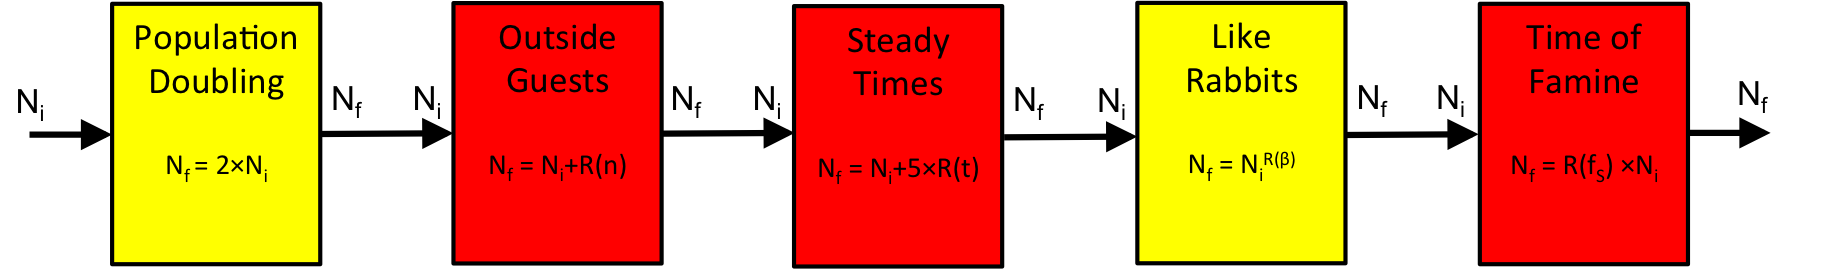
\includegraphics[width=\linewidth]{figures/toymodelflow.png}
 \caption{A pictorial representation of the layout of a population evolution model showing a number of deterministic (yellow) and stochastic (red) stages.  The rule that transforms the incoming initial population $N_i$ to the final population $N_f$ at each stage of the process is indicated in the respective box and, as indicated, the final population from the $i$-th stage is used as the initial population for the $i+1$-th stage of the evolution. }
 \label{fig:mc_chain}
\end{figure}

To proceed through each of the steps of the model of this process, the rule that is described is quantified and then applied to the existing state of the system, in this case the population.  In some cases, the same thing will occur, in which case the rule is applied in the same way.  In other cases, there is a stochastic element which necessitates for the application of the rule to determine an exact value for a random number.  If the model being implemented calls for uniformly distributed random numbers, the manner in which these are obtained is straightforward [ADDREF] and it can always be assumed that the generation of an ensemble of numbers uniformly distributed between [0,1] can be obtained easily~\footnote{In python, this is done via the \href{https://docs.python.org/2/library/random.html}{\texttt{random.random()}} and this is the only built in random generator function that should be used throughout the tutorial.}.  However, in some cases, the transformation that occurs in a stochastic stage of your model depends on random numbers that are not uniformly distributed.  As such, it is necessary to be able to select random numbers distributed according to any arbitrary probability distribution function (PDF).  Two common methods that can be used to achieve this are the \textit{accept-reject method} and the \textit{inverse transform method}.  Both of these techniques are commonly used in high energy physics and described by the particle data group in Reference~\cite{pdg_mctechniques} but provided here is a short summary of them.

\begin{center}
\fbox{\begin{minipage}{6in}
Practice writing a program in~\textsc{Python} that generates random numbers.  In the first case, write a program to generate 1000 random numbers distributed uniformly between [0,1] and make a histogram of these numbers.  In the second case, write a program that distributes the random numbers between [5,15] and makes a histogram.  Remember, it is only allowed to use the \href{https://docs.python.org/2/library/random.html}{\texttt{random.random()}} functionality in~\textsc{Python}.  As a hint, think about how to make the minimum and maximum of the [0,1] distribution into the minimum and maximum of the [5,15] distribution.
\end{minipage}}
\end{center}

\subsection{Intermezzo : Documentation and Version Control}
You may be working through this tutorial with your main interest being in particle physics.  That is great!  However, much research in particle physics, in particular the kind you will learn here, involves data analysis through the use of programming.  Therefore, to start off on the right foot and build good habits in your work, all of your work should be documented and version controlled on \href{https://github.com/}{\textsc{GitHub}}.  The reason that we do this, and use a service like \textsc{GitHub} is to ensure two main things 

\begin{enumerate}
\item ``Sharing is good!'' : Our code is well-documented and accessible to the outside world.  
\item ``Oh \$*@T!'' : If your hard drive crashes, you lose your laptop, or accidentally type \texttt{rm -rf ~/*} into the terminal, you are not screwed.
\end{enumerate}

If this is a new concept to you, then do not skip this section.  Instead, follow \href{https://try.github.io}{this Git tutorial} and register for an account on \textsc{GitHub}.  Once you are more familiar with how to use \textsc{Git}, another good tutorial can be found at \href{http://learngitbranching.js.org/}{this second Git tutorial}.  After that, all of the work that you share with collaborators should follow these simple guidelines :

\begin{itemize}
\item Do not email your code to people.  If your code is worth sending to someone else, it should be accessible by sharing a link like \href{https://github.com/smeehan12/PythiaSimulatorAnalysis}{https://github.com/smeehan12/PythiaSimulatorAnalysis} in an email.  
\item Include a \textsc{README} file.  This file should include (\textit{i}) a description, (\textit{ii}) a list of authors, (\textit{iii}) a set of directions to follow to run the code, (\textit{iv}) a description of the expected output from the code.
\item Do not send untested code.  Before sending your code to someone else to use, you should test the code as if you were them.
\end{itemize}

If you follow these rules and build habits, you will be a much more enjoyable individual with which to work.


\subsection{Accept-Reject Monte Carlo}
The accept-reject method, sometimes called the Von-Neumann method, can best be understood by examining a random process of making a measurement of a truly random physical system, that being a quantum mechanical particle in a box in a well-defined single Eigen state of the ground state energy as in Figure~\ref{fig:particle_in_box_1}.  


\begin{figure}
 \centering
\subfloat[]{
 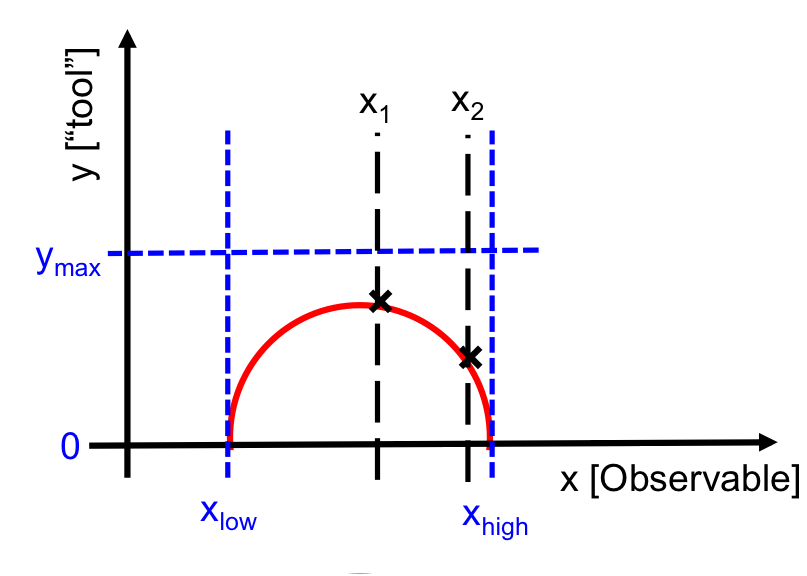
\includegraphics[width=0.3\linewidth]{figures/qm1.png}
 \label{fig:particle_in_box_1}
}
\subfloat[]{
 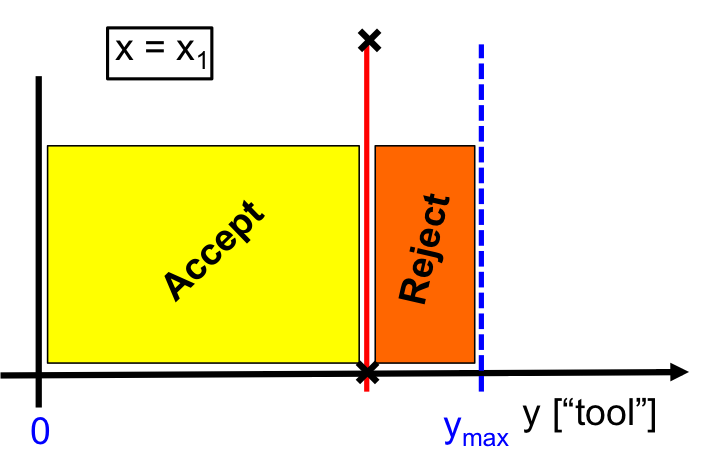
\includegraphics[width=0.3\linewidth]{figures/qm2.png}
 \label{fig:particle_in_box_2}
}
\subfloat[]{
 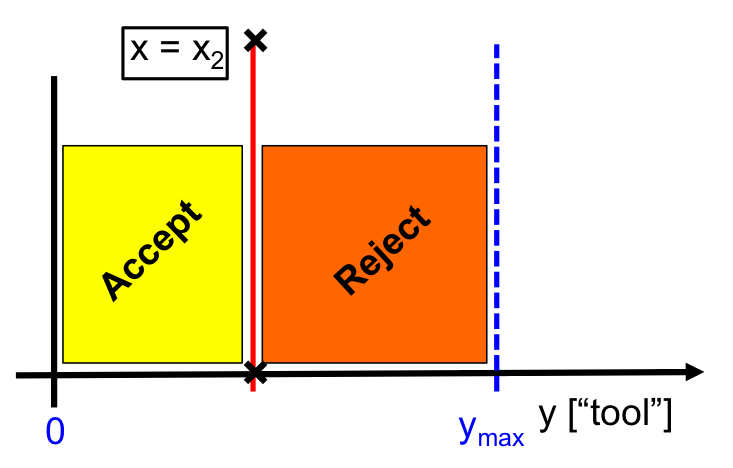
\includegraphics[width=0.3\linewidth]{figures/qm3.png}
 \label{fig:particle_in_box_3}
}
 \caption{A cartoon representation of the implementation of the accept-reject Monte Carlo generation method to produce a single $x$ measurement from the ground state of a particle in a box system in quantum mechanics.  The ground state probability density function (left) with the observable bounds $x_{low}$ and $x_{high}$ and two example random $x$ values $x_1$ and $x_2$.  Also shown are the decision making tools for single generations of $x_1$ (middle) and $x_2$ (right) showing the $y$ values for which the given $x$ value is accepted and rejected.}
 \label{fig:particle_in_box_acceptreject}
\end{figure}

In this scenario, the measurement of interest which will be the randomly distributed observable is the position of the particle in the box $x$.  In this case, the set of measurements that is produced should be distributed according to the wave function of the system~\footnote{Actually, if the wave function is $\Psi(x)$ then they will be distributed according to the probability density $|\Psi(x)|^2$.} which gives the probability of where the particle is, and when performing a measurement (i.e. draw a random value for $x$) it becomes a specific instance of that location.  Finally, we wish to make many measurements and wish to obtain an ensemble of $x$ measurement values.  However, in order to generate a measurement the position of the particle, it is actually necessary to generate two numbers, both the observable of interest $x$ and an auxiliary random number ``tool'' which we will call $y$.  For the purpose of simplicity, for now you can generate them from uniformly random distributions distributed between 0 and 1.  This imposes a few constraints on where the particle is by constraining $x$ to be between [0,1] but an ensemble of such events will not be distributed according to the wave function.  To obtain an ensemble of $x$ values that are distributed according to that constraints, you need to be clever about choosing which instances of $x$ to keep in the ensemble and which to not keep.  

To achieve this, we will use $y$.  The value $y$ has nothing to do with physics (unlike $x$ which represents the location of the particle in the box).  Instead, $y$ can be viewed as nothing more than a tool which allows you to either ``accept'' the event and collect it into part of your ensemble of events, or ``reject'' the event and think no more of that specific instance of the choice of $x$.  You want to preferentially keep $x$ values that are close to the center of the box but also sometimes keep events in the tails.  To do this, think about taking a single slice in $x$ near the tail as in Figure~\ref{fig:particle_in_box_2}.  Whenever you draw an $x$ value here, you must draw a corresponding $y$ value and compare it to the value of the function $PDF(x)$.  Since its in the tail, its more likely that the $y$ value chosen at random is larger than the function value.  Therefore, if you were to throw away the $x$ values here when the corresponding random $y$ is greater than $PDF(x)$, you will only be left with a few $x$ values with this value in your ensemble.  However, if instead you were to be looking near the center of the distribution, as in Figure~\ref{fig:particle_in_box_3}, then the situation is different.  More of the time, $PDF(x)$ is greater than $y$ so you are forced to keep a larger fraction of these events.  But, the value of $y$ that you choose must always be able to allow for the possibility of either accepting \textit{or} rejecting a given $x$ value.  So the range of $y$ values must be chosen to extend at least to the maximum value of the function.  As such, if the functional form of the probability density function has a maximum value that is greater than 1, then the range over which the $y$ value is chosen must be extended to encompass the full function.  If it extends above the maximum value of $PDF(x)$ in the range of interest, that is fine, but then the overall fraction of throws of $x$ that you accept will be smaller and your generation of accepted Monte Carlo events will be less efficient.

\begin{center}
\fbox{\begin{minipage}{6in}
Practice writing a program in~\textsc{Python} that generates random numbers, distributed according to a Gaussian distribution with a mean $\mu$ of 5 and a width $\sigma$ of 2 in the range of [0,10].
\end{minipage}}
\end{center}

Another explanation of the accept reject method is provided in Reference~\cite{acceptreject_video}.

\subsection{Inverse Transform Method}
A complementary method to the accept-reject method is the inverse transform method and aims to achieve the same goal, generating an ensemble of measurements, $x$ values, that are distributed according to some generic probability distribution function.  However, there exist a number of differences that make this method markedly different in how it achieves this goal.  

To understand how the algorithm proceeds and examine the differences with respect to the accept-reject method, we will again use the example of a particle in a box in the ground state.  In this case, the ground state PDF is as shown in Figure~\ref{fig:particle_in_box_4} and we desire to generate an ensemble of $x$ values that are preferentially located near the center of the box.  The first step is to \textit{transform} the PDF to the cumulative density function (CDF) by integrating the PDF from 0 to $x$ to obtain $CDF(x)$ as in Figure~\ref{fig:particle_in_box_5}.  It is this CDF which will be used in the generation of accepted $x$ values by using it as a translation tool.  To achieve this, you again start with the generation of uniformly distributed random numbers using \href{https://docs.python.org/2/library/random.html}{\texttt{random.random()}}.  However, in this case, these values will be used as the $y$ values to begin with, however instead of comparing these values to the PDF, these initial $y$ values will be translated to accepted $x$ measurement values by finding the \textit{inverse} of the CDF by inverting the formula $CDF(x)=y$.  Because the CDF is one-to-one, by construction this $x$ value is uniquely defined and is directly taken as the observed measurement.  

\begin{figure}
 \centering
\subfloat[]{
 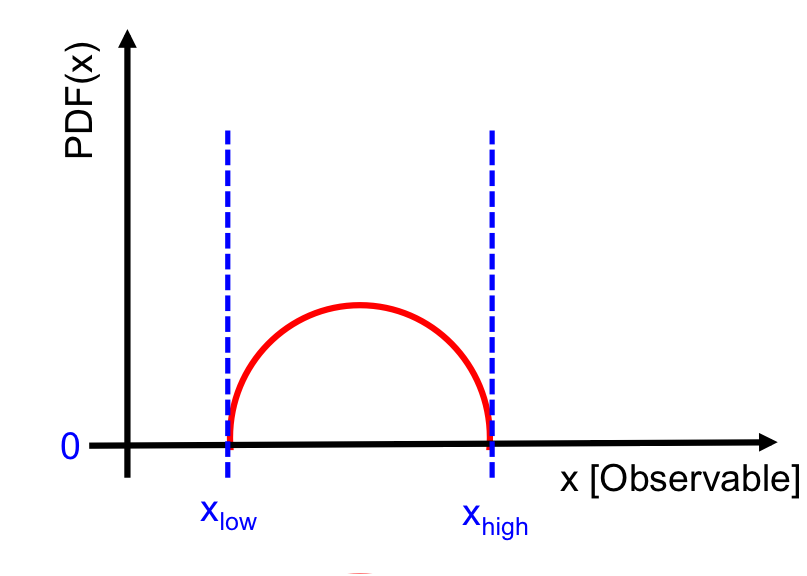
\includegraphics[width=0.3\linewidth]{figures/qm4.png}
 \label{fig:particle_in_box_4}
}
\subfloat[]{
 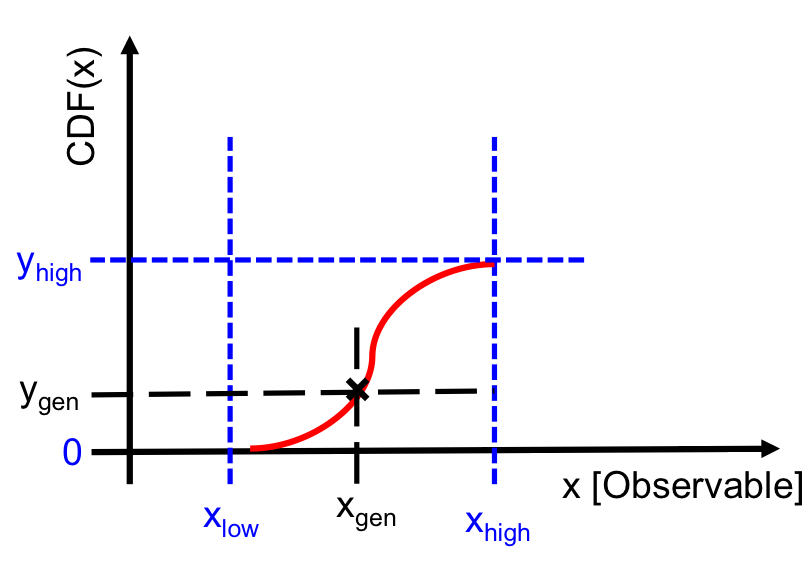
\includegraphics[width=0.3\linewidth]{figures/qm5.png}
 \label{fig:particle_in_box_5}
}
 \caption{A cartoon representation of the implementation of the iverse-transform Monte Carlo generation method to produce a single $x$ measurement from the ground state of a particle in a box system in quantum mechanics.  (Left) The ground state probability density function (left) with the observable bounds $x_{low}$ and $x_{high}$ corresponding to 0 and $y_{high}$ on the cumulative probability density function (right).  Also shown is the generation of a single observation by the generation of a random value $y_{gen}$ and translation to the observed value $x_{gen}$.}
 \label{fig:particle_in_box_inversetransform}
\end{figure}

\begin{center}
\fbox{\begin{minipage}{6in}
Reason for yourself, conceptually, how the generation of a uniformly distributed set of events on the $y$ axis is correctly translated to a set of events distributed according to the PDF.  Specifically why is the translation function chosen to be the CDF?  Is it possible to choose another functional form and achieve the same result? It may help to address this question with a picture.
\end{minipage}}
\end{center}

Finally, it is necessary to carefully tune the range of generated $y$ values to give the desired range in $x$ for the ensemble of observations.  This is rather straightforward and is achieved by starting with the desired $x$ range [$x_1$,$x_2$] and translating it to the necessary $y$ range [$y_1$,$y_2$]=[$CDF(x_1)$,$CDF(x_2)$].  

In this case, there is the advantage that for each accepted measurement $x$, only a single random number must be generated.  Moreover, the fraction of generated random numbers that are kept as accepted events is 100\% and therefore fully efficient.  This is in contrast to the accept-reject method in which the efficiency of the algorithm, depending on the functional form of the PDF, can be very small.  However, there is an additional step that is not required in accept-reject, being the evaluation of the CDF from the PDF.  In this example, the PDF of the ground state system is $PDF(x)~sin(x)^2$ and so the CDF can be evaluated analytically to give a complete formula for the CDF.  In cases where the PDF is not as well defined, or perhaps not even analytically defined, this transformation can be done numerically to obtain a piecewise function. 

\begin{center}
\fbox{\begin{minipage}{6in}
Practice writing a program in~\textsc{Python} that generates random numbers,  distributed according to a Gaussian distribution with a mean $\mu$ of 5 and a width $\sigma$ of 2 in the range of [0,10].
\end{minipage}}
\end{center}

\begin{center}
\fbox{\begin{minipage}{6in}
Practice writing a program in~\textsc{Python} that generates random numbers, distributed according to a falling distribution of the form $e^{-x}$ in the range [0,5].  After doing this, generate the same distribution using the accept-reject method and determine the efficiency of the generation, defined as the fraction of accepted $x$ values with respect to the total generated $x$ values.  How does this efficiency compare for the accept-reject method and the inverse transform method.
\end{minipage}}
\end{center}

\section{Monte Carlo Jets Model}
\label{sec:mcmodel}
As described in Section~\ref{sec:whatisjet}, one of the most commonly observed objects in an LHC collision event is a jet.  A jet itself is a collection of many particles travelling in the same general direction produced from an initial high energy parton that is produced in the event.  The process by which these particles are produced, as described in Sections~\ref{sec:ps} and~\ref{sec:had} is itself a stochastic process that centers around the concept of one-to-two splittings.  At each stage of splitting, exponentially more particles are created, but the energy of these particles monotonically decreases as the energy of the initial particle is divided more and more until the system ``freezes out'' into a collection of stable hadrons.  

In this section, we will describe a simple model for this production of the building blocks of a jet which will then be clustered using the principles in Section~\ref{sec:jetrec}.  The primary goal of this section is for you to implement the model in a \textsc{Python} or \textsc{c++} program with the only external random number generator package being that which produces uniformly distributed random numbers, as described in Section~\ref{sec:mcintro}.  The specifications for this program are that it should take as \textit{input} a single four-momentum vector, representative of an initial parton and produce as \textit{output} a collection of final state four-momentum vectors representative of the stable final state hadrons.  There are a number of free parameters that should be easily tuneable when given to a user and these are described in Sections~\ref{sec:mc_ps} and~\ref{sec:mc_had}.

\subsection{The Parton Shower}
\label{sec:mc_ps}
The parton shower model itself is a recursive process built around the idea of successive one-to-two splittings, shown in Figure~\ref{fig:splitting1}, which are chained together in a recursive tree-like sequence as in Figure~\ref{fig:splitting1}.  In this sense, the Monte Carlo model of the parton shower can be described by a sequence of only two stochastic and deterministic processes

\begin{itemize}
\item Deterministic : A particle produced with some four-momentum $(E,p_x,p_y,p_z)$ travels for a finite amount of time $t$ and traverses some distance, determined by its kinematics and the travel time\footnote{In a real collision, no finite observable distance is traversed.  This stage of the model is included for visualization purposes.}.
\item Stochastic : After this travel time, the particle decays by the emission of a radiative particle at an angle $\theta$ with respect to the initial direction of travel with a fraction $z$ of the energy of the initial particle.  
\end{itemize}

\begin{figure}
\centering
\subfloat[]{
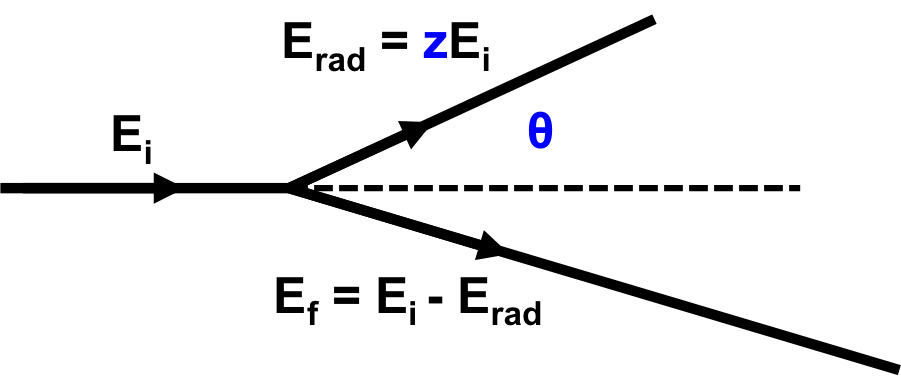
\includegraphics[width=0.4\linewidth]{figures/singlesplitting.png}
\label{fig:splitting1}
}
\subfloat[]{
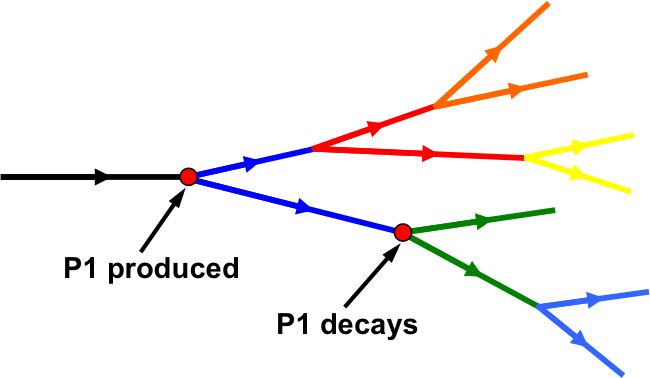
\includegraphics[width=0.4\linewidth]{figures/fullshower.png}
\label{fig:splitting2}
}
\caption{A single one-to-two splitting (left) highlighting the stochastic observables in the process and the composition of multiple splittings to form a full parton shower (right).}
\label{fig:splitting1}
\end{figure}

To implement this recursive model, it is necessary to understand more completely both of these base processes.  The deterministic stage which, in Figure~\ref{fig:splitting2}, brings particle P1 from the initial location, where it was produced by the initial radiative decay, to the final location, where it too will decay, is calculable from relativistic kinematics.  

The details of the process of a decay, the one-to-two splitting, must be treated with more care, and where possible, simplified.  As described in Section~\ref{sec:ps}, the exact way this splitting occurs depends on the initial and final state particles.  However, we will start by making the simplification to treat all splittings in the same way.  As such, there are only two parts of this stage of the model that are stochastic, the angle of emission and the energy of the emission.  As discussed in Section~\ref{sec:ps}, the physics of QCD produces soft and collinear splittings and so the PDFs of these observables should follow the functional forms

\begin{itemize}
\item $z$ (soft$~\frac{1}{z}$) : This can be seen to have a singularity at $z=0$ and therefore must be slightly modified to either ($i$) have a finite value at $z=0$ by setting $PDF(z)=\frac{1}{1+z}$ and allowing the range of possible $z$ values to span [0,1] or ($ii$) setting $PDF(z)=\frac{1}{z}$ and setting a lower minimum bound on the allowable $z$ values as [$\epsilon_z$,1].  Either is fine, and is a specific choice of your model.
\item $\theta$ (collinear$~\frac{1}{\theta}$) : This can be seen to have a singularity at $\theta=0$ and therefore must be modified in a similar way as for $z$.  However, the range of $\theta$ is slightly different and should vary between [0,$\pi/2$].
\end{itemize}

In a given splitting, after generating a random ($z$,$\theta$) pair, the kinematics of the radiated particle are determined.  However, to continue the shower process and allow for the model to proceed it is necessary to determine the kinematics of the final state particle, from which the radiation was emitted.  At this point, with one simplifying assumption, and by applying the conservation of energy and momentum, the final state kinematics of both outgoing particles.  

\begin{center}
\fbox{\begin{minipage}{6in}
Can you determine which simplifying assumption it is that allows for the full determination of the final state?  The main point is to recognize the energy scales we are talking about here in comparison to the typical energy scale of stuff at the LHC ($~$TeV).
\end{minipage}}
\end{center}

This same type of splitting, but with different random ($z$,$\theta$) pairs can then be linked together in a sequence to generate a pictorial representation of this two dimensional shower structure as in Figure~\ref{fig:splitting2}.

\begin{center}
\fbox{\begin{minipage}{6in}
This parton shower model should be implemented such that, in addition to the output set of four-momentum vectors, a graphical representation of the parton shower tree is produced from your program.  This takes careful organization of the flow of information and can be achieved in multiple ways.
\end{minipage}}
\end{center}

The entire description of the parton shower model thus far has implicitly assumed that the kinematics are constrained to two dimensions and are in a two-dimensional plane.  Since the real physics we care about modelling is in three dimensions, we need to modify the stochastic portion of the process model to account for this.  This is achieved by including an additional splitting angle $\phi$ which is the azimuthal angle of the decay around the direction of travel of the initial particle, as shown in Figure~\ref{fig:azimuth}.  However, given the structure of the QCD interaction described in Section~\ref{sec:ps}, there is no preference for the value of this angle and it should therefore be chosen from a uniform distribution with a  range of [0,$\pi$].  

\begin{figure}
\centering
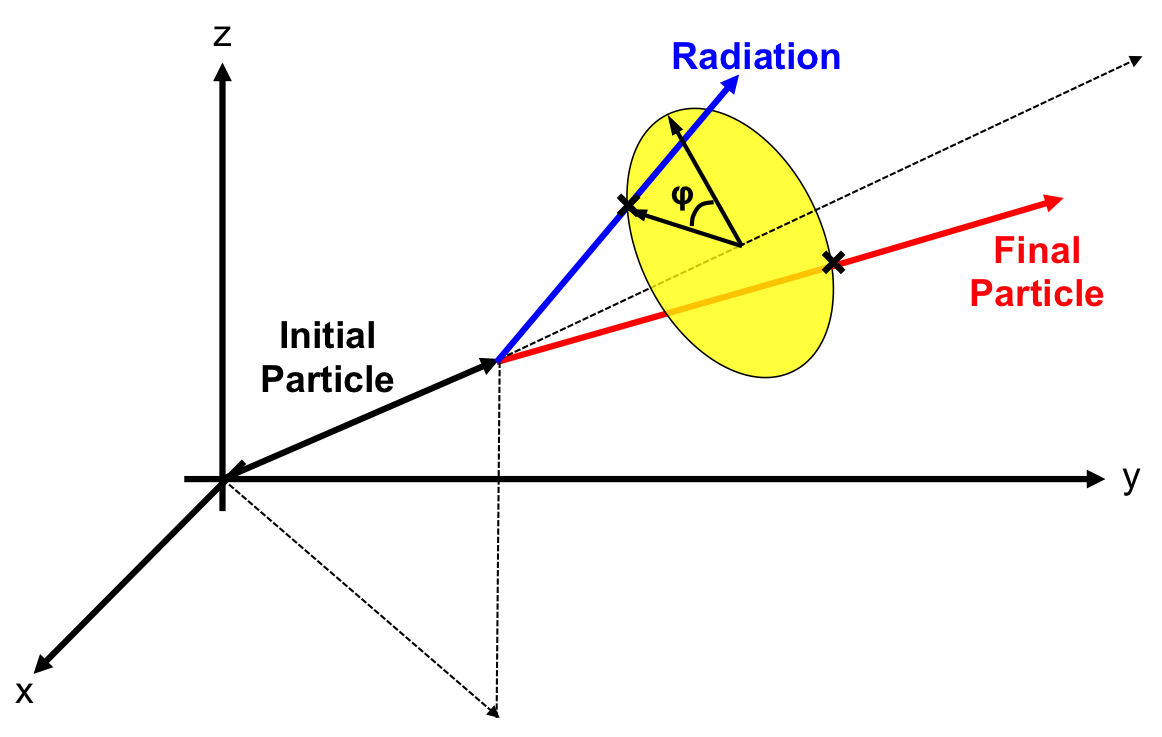
\includegraphics[width=0.7\linewidth]{figures/azimuth.png}
\caption{A illustration of the azimuthal angle $\phi$ of a one-to-two splitting occurring in three dimensions.}
\label{fig:azimuth}
\end{figure}

It is acceptable to proceed through Section~\ref{sec:mc_had} working in two dimensions.  This can help to build intuition and make the validation of your process model simpler.  However, it is necessary to include the full three dimensional model, as described here, before proceeding to Section~\ref{sec:jetrec}.


\subsection{Hadronization}
\label{sec:mc_had}
As described in Section~\ref{sec:had}, the parton shower proceeds until the energy scale of the individual particles decreases to the point where it is energetically favorable to form stable hadrons with other partons existing within the event.  The manner in which this happens is not well understood from first principles and for this model, we will take a very simple approach and making a direct translation between each parton and each hadron.  To achieve this, choose an energy scale threshold $E_{crit}$ below which a parton that has been radiated or continuing from the initial splitting does not split further.  This should be made a parameter that is easily tunable in a single location within your program.

\section{A Jetty Event}
\label{sec:event}
In LHC collision, it is very rare to produce a single parton in the hard collision.  More often than not, two partons will be emitted.  Now, because the collision was between two particles travelling opposite to each other, we will make the simplifying assumption that the initial state was completely balanced and had an initial momentum of $p_{initial}=0$.  Therefore, when the two partons are emitted, they must be in a configuration that obeys the conservation of momentum (i.e. ``back-to-back'').  However, there are some aspects of this configuration which are stochastic, namely :

\begin{itemize} 
\item Energy : The actual energy of one of the emitted partons is random and distributed according to an exponentially falling distribution $e^{-\alpha E_{parton}}$ where $\alpha$ is a physically meaningful parameter that characterizes collisions at the LHC and $E_{parton}$ is the randomly chosen energy of the parton.
\item Azimuthal direction : The collisions that occur have no preferred direction in terms of the azimuthal angle $\phi$ as shown in Figure~\ref{fig:direction_event}.  Therefore, this is a randomly distributed observable with a flat distribution from [0,$2\pi$].
\item Polar direction : Again, the collisions that occur have no preferred direction for the emissions and so the polar angle $\theta$ in Figure~\ref{fig:direction_event} is a random number distributed evenly from [0,$\pi$].
\end{itemize}

\begin{figure}
\centering
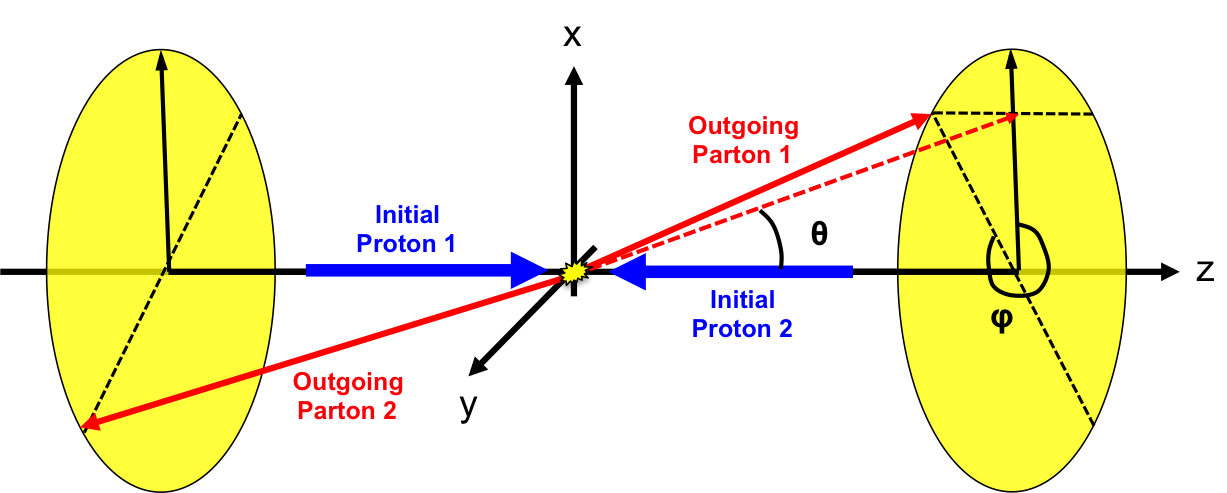
\includegraphics[width=0.4\linewidth]{figures/jettyevent.png}
\label{fig:direction_event}
\caption{A pictorial representation of a proton-proton collision event similar to that occurring in the LHC.  Shown here are the incoming protons and the two outgoing partons with the topology specified by the polar angle $\theta$ and azimuthal angle $\phi$.}
\label{fig:direction_event}
\end{figure}

\begin{center}
\fbox{\begin{minipage}{6in}
In Section~\ref{sec:mcmodel}, a single parton with an initial hard-coded four vector momentum of a parton $P$  was sent through the parton shower and hadronization to produce a collection of particle pseudojets $p_i$ like $P\rightarrow [j_1,j_2,...,j_n]$.  Augment this by initially producing an \textit{event} with the properties described here and then showing both of the partons in the collision.  Procedurally, you will have to produce two initial partons $P^a$ and $P^b$ and then shower each independently as $P^a\rightarrow [j^a_1,j^a_2,...,j^a_n]$ and $P^b\rightarrow [j^b_1,j^b_2,...,j^b_n]$.  Finally, you should take the union of these final state particles to produce the full showered event.
\end{minipage}}
\end{center}

\section{Jet Reconstruction}
\label{sec:jetrec}
The simulation that you have written in Section~\ref{sec:mcmodel} represents the evolution of a single energetic parton to many low energy stable hadrons.  Conceptually, this is the process that occurs after a proton proton collision emits a parton which produces the collimated sprays of particles that are observed in the detector.  However, this is not yet a jet.  Even though all particles originated from the same parton, there is a level of ambiguity due to the recursive structure of the shower.  This can be seen from the first splitting in the tree.  After this splitting, the system contained not one parton, but two.  At this point, the intuition of ``\textit{jet=parton}'' would lead us to believe that there should be two jets in this (pseudo)event.  So which notion is correct?  Is there one jet or two?

To resolve this ambiguity, it is necessary to concretely define what is meant by collimated spray and this is done via a \textit{jet clustering algorithm}.  A full review of these algorithms (and much more) is provided in Reference~\cite{Ellis:2007ib} but all achieve the same aim of partitioning the full set of stable final state particles into subsets of particles using a set of rules based on the intuition of what a ``collimated spray'' actually is.  After performing this clustering, the concept of a jet is fully defined and it is possible to quantify features of this jet by designing observables to study how the jet was formed in the parton shower or to highlight defining features to classify the initial type of particle from which the jet originated.



\subsection{Jet Finding}
The idea that a collimated spray of hadrons in the detector is representative of an initial high energy parton is only useful if it is possible to concretely define a collimated spray.  This is done by clustering algorithms that take as input a collection of four-momentum vectors from an entire event (which themselves may originate from multiple partons as described in~\ref{sec:event}) and return subsets of four vectors with each of these subsets being a ``jet''.  The way in which these subsets are defined has evolved over time~\cite{Ellis:2007ib} and at the LHC, the most commonly used clustering algorithms that are used rely on the concept of \textit{iterative recombination}~\cite{Cacciari:2008gp}\footnote{The primary reason that these algorithms are preferred is because they are (i) infrared and (ii) collinear (IRC) safe, meaning that they are invariant under the presence of additional infinitely soft radiation in the event or an additional infinitely collinear one-to-two splitting in the parton shower.  In some sense, this can be thought of as being robust against the exact details of the parton shower, which themselves are only approximation of the true physics.}.  The intuition that drives these algorithms can be thought of as a reversal of the model created for the parton shower.  Therefore, instead of starting with one particle and performing one-to-two splittings until you have many low energy particles, these algorithms start with many low energy particles and perform pairwise two-to-one combinations until you have ``sufficiently distinct'' four momentum collections.

This clustering process begins with the set of final state particles.  In the case of the simulation here, these are the real particles coming from the hadronization process but in an actual experiment these will be observed and reconstructed signals in the detector, such as calorimeter clusters or charged particle tracks.  At this point, it is also helpful to regard the particles as pseudojets, which are four-momentum vectors at an intermediate stage of the clustering process which themselves may be composed of previous combinations of pseudojet four momentum vectors. The order of the pairwise clustering combinations the decision that a given collection (pseudojet) is sufficiently distinct from the others then proceeds by following a set of abstract distance metrics\footnote{In this context, distance does not mean physical distance of length measured in meters.  Remember, the entire parton shower and hadronization process occurs in an unimaginably small distance.}.  The first, $d_{ij}$, measures the distance between any two pseudojets in the event.  This distance is defined in Equation~\ref{eqn:dij} and takes into consideration both the energy of the particles that may be combined by using their transverse momentum \pt and the angular distance $\Delta_{ij}=\sqrt{(\phi_i-\phi_j)^2+(\eta_i-\eta_j)^2}$\footnote{} separating them.  The second, $d_{iB}$, is commonly referred to as the \textit{beam distance} and provides a measure of the distinctness of any given pseudojet $i$ from the rest of the clustered event and is defined in Equation~\ref{eqn:dib}.

\begin{equation}
\label{eqn:dij}
d_{ij}=min(p_{Ti}^{2n},p_{Tj}^{2n})\times \frac{\Delta_{ij}}{R}
\end{equation}
\begin{equation}
\label{eqn:dib}
d_{iB}=p_{Ti}^{2p}
\end{equation}

For a given stage of clustering, whether it be the initial stage when there are $N$ initial single particle pseudojets or later when some of these have been bundled together into some lesser number of composite pseudojets, all possible distance measured are calculated.  This will produce $N$C$2$ pseudojet pseudojet distances and $N$ pseudojet-beam distances.  From the full set of distances, the minimum distance dictates the action that is to be taken in the clustering sequence.  In the case that the minimum distance is a $d_{ij}$ distance, it can be interpreted as indicating that in the event, the next best thing to do is group those two particles, $i$ and $j$, together as having originated from a common one-to-two splitting in the parton shower.  Conventionally, this grouping is done by simply adding together the four-momentum vectors of these constituents to obtain some resultant four vector.  If, on the other hand, the minimum distance is a $d_{iB}$ beam distance, then the interpretation is that there exists a pseudojet in the event\footnote{Note that this pseudojet can itself be a single particle or a pseudojet composed of multiple pairings due to previous $d_{ij}$ combinations.} is distinct enough that it should be interpreted as representing a hard parton originating from the underlying physics process.  In this case, the pseudojet is set aside and becomes a jet.

In both of these cases, either an $ij$ combination or the promotion of a pseudojet $i$ to a jet, the number of pseudojets in the event decreases by one.  Therefore, the algorithm proceeds in this iterative fashion until all pseudojets have been promoted to some jets and there exist no more pseudojets for clustering.

\begin{center}
\fbox{\begin{minipage}{6in}
From the previous Monte Carlo model you have created, you have the ability to simulate parton showers/hadronizations that are representative of hadronic activity in LHC collisions.  At this stage, implement the \antikt algorithm to cluster a single event, including proper validation of the procedure.  Note that you will have to specify the parameters $n$ and $R$ which are choices of the algorithm.  Make a histogram of the number of jets that result from this algorithm for 1000 parton showers and do this for the set of $n$ values of [-1,0,1] and $R$ values of [0.01,0.05,0.1,0.5,1.0].  What differences do you see?  Do they make sense?
\end{minipage}}
\end{center}

\begin{center}
\fbox{\begin{minipage}{6in}
The algorithm described here is commonly referred to as \textit{inclusive jet finding}.  A complementary algorithm, called \textit{exclusive jet finding}, exists that performs clustering in a slightly different way and truncates based on a different condition.  Find a description of this algorithm and compare and contract it to inclusive jet finding.  Implement this algorithm in your program such that it is possible to cluster jets in either fashion.
\end{minipage}}
\end{center}


\subsection{Jet Observables}
After having performed jet clustering on the generated parton shower, there exist a set of jets that themselves are exclusive subsets of the initial set of stable particles resulting from the parton shower and hadronization.  In principle, they are representative of a hard parton in the event and because they were formed by combining four-momentum vectors together, it is possible to make the association $(E,p_x,p_y,p_z)_{parton}\sim (E,p_x,p_y,p_z)_{jet}$.  Focusing on the 0$^{th}$ entry of this four vector and noting that the jet itself is composed of multiple particles from the parton shower, one can recognize that the parton energy is represented as $E_{parton}\sim E_{jet}=\sum_{i\in \text{jet constituents}}E_{i}$ where the \textit{jet constituents} are the stable particles that the jet clustering initially started with.  Viewing one component of the jet four vector this way is an example of a single jet \textit{observable}.

However, it is possible to generalize this concept of a jet observable to be any function that takes as an argument the set of jet constituents and produces a single scalar quantity.  Explicitly, this is $O(jet)=function([j_1,j_2 ,...,j_n])$ where $j_i$ are each of the $n$ four vector measurements of the initial single particle pseudojets.  Implementing this is challenging from the organizational standpoint as it requires you to keep track of the initial four vectors as the clustering proceeds, not just the combined four vectors.  The exact form of $function()$ is chosen based on the intuition of some physical property of the parton or jet that one is interested in summarizing in a way that can be formed into a one dimensional spectrum.  In the case of the jet energy, the interpretation of the feature of the jet is direct and represents simply the amount of energy that the initial parton had when produced by the physics process.  However, more complicated observables can be formed that quantify and can be used to investigate features of the parton shower model that was initially implemented in Section~\ref{sec:mcmodel}.  Perhaps most importantly though, the quantification of a jet feature in this way can be done both in Monte Carlo simulation and in real collision data, allowing for the measurement or tuning of the underlying parameters of the model used to generate the parton shower.

\begin{center}
\fbox{\begin{minipage}{6in}
Based on the jets that you have clustered in the previous section, calculate the  jet ``pseudo-mass'' as 
\begin{center}
$\text{SimpleMass}(J) = E(j_1)\times E(j_2)\times \Delta R(j_1,j_2)$
\end{center}
where $j_1$ and $j_2$ are the two highest \pt constituents of the jet $J$.  In the case that a given parton shower and clustering produces more than one jet, perform this calculation for the jet of highest energy.  Perform this calculation for a large number of parton shower generations and make a histogram of the pseudo-mass for all of these generated showers.
\end{minipage}}
\end{center}


\section{Conclusion and Project Extensions}
\label{sec:extensions}
That brings you to the end of this tutorial.  Having worked through it, the intention is that you have learned something practical, in terms of programming, and intellectual, in terms of physics.  The next step is to start to create your own questions and define a research direction of your own.  This can be done by either building on the project you have already begun, with some suggestions provided in Section~\ref{sec:ext1} or by moving to the usage of tools more commonly used in HEP as in Section~\ref{sec:ext2}.

\subsection{Toy Monte Carlo Extensions}
\label{sec:ext1}
Described here is a list of possible extensions for the toy Monte Carlo simulation that you have written.  If you have an idea to pursue that has come up during the course of working through the tutorial, pursue that instead.  However, some of these may be interesting jump off points.
\begin{itemize}
\item \textbf{Parton Distribution Functions}~\cite{pdf1,pdf2,pdf3,pdf4} : If a proton collides with a proton, then the collisions really occur between the underlying constituents, the quarks and gluons.  Because the physics that can result from a given type of collision (\textit{up-quark:up-quark} vs. \textit{up-quark:gluon}) differs, understanding how to incorporate this degree of randomness into the generation of an ensemble of full events is important.  In this extension you will take the jet model you built and interface it with a model of proton collisions which may produce different final states depending on the initial state.
\item \textbf{Comparing Hadronization Models} : Depending on what observable is being reconstructed, the degree of sensitivity to the details of hadronization model can vary.  And in a number of processes studied at the LHC and searches for new physics, this can become a limiting factor in terms of uncertainties.  In this extension, you will construct two hadronization models based on the principles of \textsc{Pythia} and \textsc{Herwig} and compare a number of observables.
\item \textbf{Detector Simulation} : After a jet (or any observable physics object) has been formed, it is observed in the detector that has been constructed around the interaction point.  This observation is made possible because of the known interactions of the incoming particle with the material of the detector.  Unfortunately, aspects of this are random and the particle may interact with multiple sub-detector components.  Therefore, it is important to model the detector using Monte Carlo simulation~\cite{det1}.  Some common simulation toolkits that are used to do this are \textsc{Geant}~\cite{Agostinelli:2002hh} and \textsc{Delphes}~\cite{Ovyn:2009tx}.  In this extension, you will build your own detector simulation using similar principles as those implemented in these programs.
\item \textbf{Simulating $W$ Bosons and $top$ Quarks}~\cite{Aad:2015rpa,Schaetzel:2014kha} : At the LHC, the high center of mass energy means that when massive objects are produced they can often have high kinetic energy.  If these massive objects decay to partons, then it is possible that the parton showers of these particles will merge and the paradigm of a jet being a parton breaks down.  Instead, it is necessary to treat a jet as a $W/Z/higgs$ boson or a $top$ quark.  The primary difference is that prior to the parton shower process, there will be one or two ``hard splittings'' that occur due to the decay of the massive object.  In this project, you will simulate these hard splittings and then interface the results to the parton shower jet simulator you have previously written.
\end{itemize}

\section{\textsc{Pythia}/\textsc{fastjet} Analysis Extension}
\label{sec:ext2}
In high energy physics, the tools used to perform the simulation of collisions events, the parton shower, and hadronization as well as the clustering of jets are standardized.  They are provided in packages that can be installed on your computer and built into larger analysis programs, similar to the use of the \href{https://docs.python.org/2/library/random.html}{\texttt{random.random()}} in \textsc{Python}.  This helps ensure that all people working in HEP speak a common language and can share their ideas more effectively.  In the case of the simulation of events, one of the most commonly used simulation tools is \href{home.thep.lu.se/~torbjorn/pythia81html/Welcome.html}{\textsc{Pythia}}.  Although it includes more refined models of the underlying physics, it functions on the same general principle of the program designed here.  In the case of jet clustering, there is a single package used by all of the LHC experiments called \href{fastjet.fr}{\textsc{fastjet}}.  In this case, although the working principle is the same as the algorithm you implemented in Section~\ref{sec:jetrec}, the exact implementation itself allows for the execution of jet finding to occur at a much faster rate.

In this extension, you will be provided with guidance on how to use these programs in the context of a simple simulation and analysis and then, after defining a research question, use this setup to investigate it.To start this extension, follow the directions provided in the \href{https://github.com/smeehan12/PythiaSimulatorAnalysis}{\textsc{PythiaSimulatorAnalysis}}.





%-------------------------------------------------------------------------------
% Bibliography
\printbibliography


\end{document}
